\section{Mailserver aufsetzen} 

\subsection{Betriebssystem starten}
Beim ersten Start des Raspberry öffnet sich nach kurzer Wartezeit ein graues Fenster auf blauem Hintergrund mit dem Titel ``Raspberry Pi Software Configuration Tool". 

\begin{figure}[h]
\centering
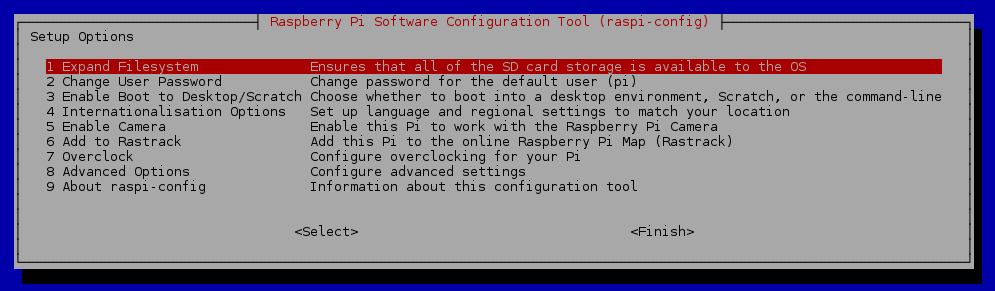
\includegraphics[scale=0.5]{images/raspiconfig}
\caption{Raspberry Pi Konfigurations-Tool}
\end{figure}

Dieses Werkzeug dient dazu, gewisse Grundeinstellungen vorzunehmen. Folgende Einstellungen sollten vorgenommen werden: 

\begin{enumerate}
\item Benutzerpasswort ändern (Change User Password)
\item Ausweiten des Dateisystems, um den Speicher der Karte voll auszunutzen (Expand Filesystem)
\item Standardumgebung einstellen auf ``Console Text console" (Enable Booot to Desktop/Scratch)
\item Anpassen des Keyboardlayouts (Internationalisation Options > Change Keyboard Layout)
\item Regionaleinstellungen auf en\_US.UTF-8 setzen (Internationalisation Options > Change Locale)
\item Zeitregion setzen (Internationalisation Options > Change Timezone) 
\item Raspberry Pi übertakten auf "Medium, 900MHz" (Overclock)
\item Speicherverteilung für die GPU auf 16 begsrenzen (in Megabyte, MB) (Advanced Options > A3 Memory Split)
\end{enumerate}

Sollte es mit den getroffenen Einstellungen zu Problemen kommen, kann das Konfigurationstool im laufenden Betrieb erneut aufgerufen werden. Folgender Befehl muss dazu in der Konsole eingegeben werden: 

\begin{lstlisting}
sudo raspi-config
\end{lstlisting} 

Sind alle Einstellungen vorgenommen, kann das Menü mittels ``Finish" verlassen werden. Die Frage, ob neu gestartet werden soll (reboot), mit "Ja" beantworten, worauf das System neu startet und alle zuvor vorgenommenen Einstellungen übernommen werden.
\\
\\
Nach dem Neustart findet man sich in einem konsolenartigen Fenster mit einem blinkenden Cursor wieder. Dies wird für den Rest des Tutorials die Arbeitsumgebung sein, da die grafische Benutzeroberfläche nicht gebraucht wird. Die Performance ist in der Konsole zudem deutlich besser.

\subsection{Root-Rechte erlangen}
Die meisten der in dieser Anleitung beschriebenen Befehle verlangen erweiterte Rechte. Diese können unter Raspbian ganz einfach erlangt werden mittels:

\begin{lstlisting}
sudo su
\end{lstlisting}

Grosse Macht bringt auch grosse Verantwortung. Hat man unter Linux Administrator-Rechte (auch Root-Rechte), kann man sehr schnell sehr vieles kaputt machen. Im schlimmsten Fall muss die SD-Karte neu aufgesetzt werden. Es lohnt sich deshalb, ein paar wenige Regeln zum Gebrauch der Konsole zu beachten: 

\begin{itemize}
\item Ein Befehl wird mittels Drücken der ``Enter-Taste" abgesetzt
\item Bevor ein neuer Befehl abgsetzt werden, muss der zuvor eingegebene abgeschlossen sein (manchmal ist Geduld gefragt)
\item Gross- und Kleinschreibung werden unter Linux unterschieden!
\item Immer sicherstellen, dass der Befehl auch wirklich richtig eingegeben wurde
\end{itemize}

\subsection{System aktualisieren}
Um sicher zu stellen, dass das System auf dem aktuellsten Stand ist, müssen zuerst alle installierten Pakete aktualisiert werden. Dazu müssen folgende zwei Befehle abgesetzt werden:

\begin{lstlisting}
apt-get update
apt-get upgrade
\end{lstlisting}

Nach der Eingabe von ``apt-get upgrade" fragt das Terminal noch einmal nach, ob man die neuen, zur Verfügung stehenden Pakete wirklich installieren will. Standardmässig ist die Antwort auf "Ja" eingestellt, was man an dem grossen Y in [Y/n] erkennt. Um fortzufahren reicht ein erneutes Drücken der ``Enter-Taste". Zukünftige Rückfragen bei abgesetzten Befehlen können auf die gleiche Weise behandelt werden. Es empfiehlt sich dennoch, die angezeigte Meldungen (Informationen, Warnungen) immer durchzulesen und entsprechend zu handeln.

\begin{figure}[h]
\centering
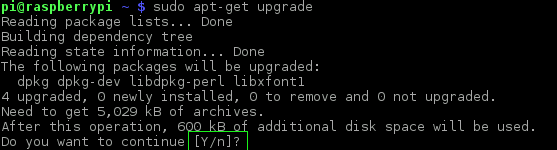
\includegraphics[scale=0.7]{images/upgrade}
\caption{apt-get upgrade}
\end{figure}

\subsection{Statische IP-Adresse}
Die IP-Adresse, durch welche der Computer im Netz eindeutig identifiziert wird, sieht möglicherweise nach jedem Computerstart anders aus. Damit der Router im Heimnetzwerk später weiss, wohin er die einkommenden Mails weiterleiten muss, sollte die IP-Adresse statisch festgelegt werden.
\\
\\
Zuerst muss die Netwerkkonfigurationsdatei unter ``/etc/network/interfaces'' angepasst werden.
\\
Dazu muss man die Datei mit einem Texteditor öffnen. Dazu kann der vorinstallierte Texeditor ``Nano" verwendet werden: 

\begin{lstlisting}
sudo nano /etc/network/interfaces
\end{lstlisting} 

\begin{figure}[h]
\centering
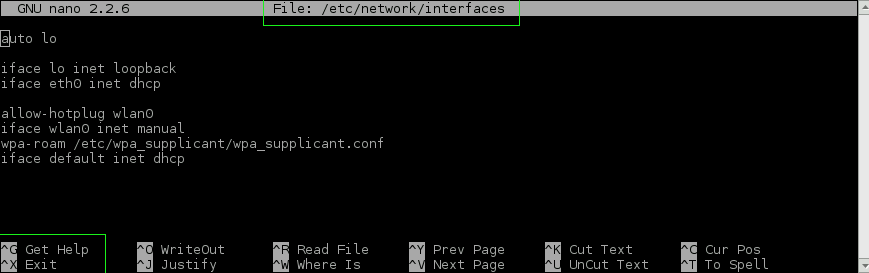
\includegraphics[scale=0.6]{images/nano}
\caption{Texteditor Nano}
\end{figure}

Unter Umständen kann es vorkommen, dass folgende Zeile bereits in der Datei steht:

\begin{lstlisting}
iface eth0 inet dhcp
\end{lstlisting}

Sofern dies der Fall ist, muss diese gelöscht und durch folgende Zeilen ersetzt werden:

\begin{lstlisting}
iface eth0 inet static
address 192.168.1.107
netmask 255.255.255.0
gateway 192.168.1.1
network 192.168.1.0
broadcast 192.168.1.255
\end{lstlisting}

Die verwendete IP-Adresse in der zweiten Zeile (192.168.1.107) sollte durch die aktuelle IP-Adresse des Systems ersetzt werden. Diese kann mit dem Kommando ``ifconfig'' ermittelt werden. Sie steht auf der zweiten Zeile bei ``eth0" unter ``inet addr:".

\begin{figure}[h]
\centering
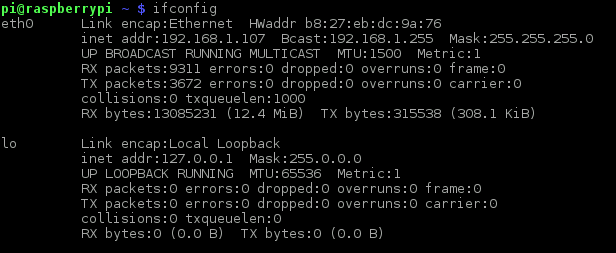
\includegraphics[scale=0.65]{images/ifconfig}
\caption{Ausgabe von ifconfig}
\end{figure}

\subsection{Voraussetzung einer Domain}
Damit ein Mailserver immer erreichbar ist, braucht es auf irgendeinem Domain Name Server einen Eintrag. Dies bedeutet, dass die Verbindung von unserem lokalen Router zu einem beliebigen anderen Computer im Internet gewährleistet ist.
... to be continued

\section{Mailordner verschlüseln}
Der Ordner, in dem später die Mails aufbewahrt werden, soll verschlüsselt werden (engl.: to encrypt). Dazu benutzt man das Programm EncFS.

Zuerst muss das Kernelmodul FUSE geladen werden. 

\begin{lstlisting}
modprobe fuse
\end{lstlisting}

Danach kann EncFS installiert werden mit: 
\begin{lstlisting}
apt-get install encfs
\end{lstlisting}

Anschliessend kann die Konfiguration vorgenommen werden. Dazu kann man einfach folgende Befehle kopieren und in der Konsole absetzen.

\begin{lstlisting}
mkdir /encrypted-mail /decrypted-mail
chgrp mail /decrypted-mail/
chmod -R g+rw /decrypted-mail/
gpasswd -a mail fuse
chgrp fuse /dev/fuse; chmod g+rw /dev/fuse
encfs /encrypted-mail /decrypted-mail -o --public
\end{lstlisting}

Bei der Frage nach dem Modus, muss man den Paranoia Mode auswählen. Einfach mittels Eingabe von p bestätigen. Danach verlangt das Programm noch das Setzen eines Passwortes. Einmal gesetzt, sollte es gut aufbewahrt werden!

\subsection{Komponenten installieren}
Als nächstes müssen alle benötigten Komponenten installiert werden.
Diese sind: 
\begin{itemize}
\item MySQL Server \\
MySQL bezeichnet eine Datenbank. Das zu installierende Paket stellt eine Datenbank für die E-Mail-Benutzer und andere Einstellungen zur Verfügung.

% FIXME: Description
\item Postfix \\
% FIXME: Description

\item Dovecot \\
% FIXME: Description

\end{itemize}

Dovecot verlangt ein aktives IPv6-Modul. Dieses muss zur entsprechenden Liste hinzugefügt und anschliessend aktiviert werden:

\begin{lstlisting}
echo "ipv6" >> /etc/modules
modprobe ipv6
\end{lstlisting}

Nun können die Pakete installiert werden:

\begin{lstlisting}
apt-get install postfix postfix-mysql dovecot-core dovecot-imapd dovecot-mysql mysql-server dovecot-lmtpd
\end{lstlisting}

Nachfolgend werden der Reihe nach für MySQL und Postfix gewisse Grundeinstellunen vorgenommen. Die Programme führen den Benutzer dabei an der Hand und gehen Schritt für Schritt die Fragen durch.

% FIXME: Screenshots einfügen + Text (caption?)

Anschliessend werden alle Pakete installiert, was ein paar Minuten dauern kann. 

Für Dovecot wird nun noch ein Passwort generiert:

\begin{lstlisting}
doveadm pw -s SHA512-CRYPT
\end{lstlisting}

Dieses wird für den ersten E-Mail-Benutzer verwendet und im nächsten Schritt in die Datenbank gespeichert.

\subsubsection{MySQL}
Zuerst muss die MySQL-Datenbank mit dem Namen "mailserver" erstellt werden. Dies geschieht mit dem folgenden Befehl:

\begin{lstlisting}
mysqladmin -p create mailserver
\end{lstlisting}

Nun wird man nach dem Passwort gefragt. Es handelt sich dabei um jenes, welches während der Installation von MySQL gewählt wurde. 

Anschliessend kann man sich in die Datenbank einloggen. Es wird erneut nach dem gleichen Passwort gefragt:

\begin{lstlisting}
mysql -p mailserver
\end{lstlisting}

Jetzt müssen alle benötigten Tabellen generiert werden:

\begin{lstlisting}
mysql> GRANT SELECT ON mailserver.* TO 'mailuser'@'127.0.0.1' IDENTIFIED BY 'mailuserpass';
mysql> FLUSH PRIVILEGES;
mysql> CREATE TABLE `virtual_domains` (
  `id` int(11) NOT NULL auto_increment,
  `name` varchar(50) NOT NULL,
  PRIMARY KEY (`id`)
) ENGINE=InnoDB DEFAULT CHARSET=utf8;
mysql> CREATE TABLE `virtual_users` (
  `id` int(11) NOT NULL auto_increment,
  `domain_id` int(11) NOT NULL,
  `password` varchar(106) NOT NULL,
  `email` varchar(100) NOT NULL,
  PRIMARY KEY (`id`),
  UNIQUE KEY `email` (`email`),
  FOREIGN KEY (domain_id) REFERENCES virtual_domains(id) ON DELETE CASCADE
) ENGINE=InnoDB DEFAULT CHARSET=utf8;
mysql> CREATE TABLE `virtual_aliases` (
  `id` int(11) NOT NULL auto_increment,
  `domain_id` int(11) NOT NULL,
  `source` varchar(100) NOT NULL,
  `destination` varchar(100) NOT NULL,
  PRIMARY KEY (`id`),
  FOREIGN KEY (domain_id) REFERENCES virtual_domains(id) ON DELETE CASCADE
) ENGINE=InnoDB DEFAULT CHARSET=utf8;
\end{lstlisting}

Die Tabellen sind jetzt bereit, um mit Daten abgefüllt zu werden. Dies sind fürs erste die Domäne und der erste Benutzer.

\begin{lstlisting}
mysql> INSERT INTO `mailserver`.`virtual_domains`
  (`id` ,`name`)
VALUES
  ('1', 'yourdomain.com');
mysql> INSERT INTO `mailserver`.`virtual_users`
  (`id`, `domain_id`, `password` , `email`)
VALUES
  ('1', '1', '$6$YOURPASSWORDHASH', 'pi@yourdomain.com');
\end{lstlisting}

% FIXME: explain pi@yourdomain.com

\$6\$YOURPASSWORDHASH muss dabei mit dem Hashwert ersetzt werden, welcher durch "doveadm pw -s SHA512-CRYPT" generiert wurde. Es muss der ganze Wert ab "\$6\$" verwendet werden.

MySQL ist fertig eingerichet und kann verlassen werden:

\begin{lstlisting}
mysql exit
\end{lstlisting}

\subsubsection{Postfix}
Nach MySQL ist jetzt Postfix an der Reihe.

Zuerst sollte man sicherheitshalbers ein Backup der originalen Postfix Konfiguration machen, sodass im Falle einer Fehlkonfiguration noch eine funktionierende vorhanden wäre. 

\begin{lstlisting}
cp /etc/postfix/main.cf /etc/postfix/main.cf.orig
\end{lstlisting}

Wurde das Backup erfolgreich erstellt, kann Postfix konfiguriert werden. Damit die Kommunikation verschlüsselt von Statten geht, müssen die TLS Einstellungen geändert werden.
Dazu öffnet man ``/etc/postfix/main.cf'' mit einem Texteditor (hier Nano):

\begin{lstlisting}
nano /etc/postfix/main.cf
\end{lstlisting}

Als erstes müssen alle Parameter unter ``# TLS Parameters" auskommentiert werden. Dies geschieht mittels einfügen einer Raute (#) vor jeder Zeile.

Nun fügt man unter den auskommentierten Zeilen folgende hinzu:

\begin{lstlisting}
smtpd_tls_cert_file=/etc/ssl/certs/dovecot.pem
smtpd_tls_key_file=/etc/ssl/private/dovecot.pem
smtpd_use_tls=yes
smtpd_tls_auth_only = yes
smtp_tls_security_level = may
smtp_tls_loglevel = 2
smtpd_tls_received_header = yes
\end{lstlisting}

Nach den TLS-Parametern müssen nun noch folgende Parameter hinzugefügt werden:

\begin{lstlisting}
smtpd_sasl_type = dovecot
smtpd_sasl_path = private/auth
smtpd_sasl_auth_enable = yes
smtpd_recipient_restrictions = permit_sasl_authenticated, permit_mynetworks, reject_unauth_destination
\end{lstlisting}

Die TLS-Parameter sind für die sicher Kommunikation zuständig (Verschlüsselung)
\footnote{\url{https://de.wikipedia.org/wiki/Transport\_Layer\_Security}}.
\\
\\
Weiter muss der Parameter ``mydestination" auf ``localhost" gesetzt werden. Alle anderen Werte muss man entfernen:

\begin{lstlisting}
mydestination = localhost
\end{lstlisting}

Zu guter Letzt müssen am Ende des Files noch folgende Zeile hinzugefügt werden:

\begin{lstlisting}
virtual_transport = lmtp:unix:private/dovecot-lmtp
virtual_mailbox_domains = mysql:/etc/postfix/mysql-virtual-mailbox-domains.cf
virtual_mailbox_maps = mysql:/etc/postfix/mysql-virtual-mailbox-maps.cf
virtual_alias_maps = mysql:/etc/postfix/mysql-virtual-alias-maps.cf
local_recipient_maps = $virtual_mailbox_maps
\end{lstlisting}

Diese stellen eine Verknüpfung von Postfix mit MySQL und Dovecot her.

Nun müssen noch die Files erstellt werden, die weiter oben in der Datenbank in Form von Tabellen spezifiziert wurden. Dazu öffnet man jedes der Files mit Nano und fügt die entsprechenden Zeilen hinzu: 

\begin{lstlisting}
nano /etc/postfix/mysql-virtual-mailbox-domains.cf
\end{lstlisting}

\begin{lstlisting}
user = mailuser
password = mailuserpass
hosts = 127.0.0.1
dbname = mailserver
query = SELECT 1 FROM virtual_domains WHERE name='%s'
\end{lstlisting}

\begin{lstlisting}
nano /etc/postfix/mysql-virtual-mailbox-maps.cf
\end{lstlisting}

\begin{lstlisting}
user = mailuser
password = mailuserpass
hosts = 127.0.0.1
dbname = mailserver
query = SELECT 1 FROM virtual_users WHERE email='%s'
\end{lstlisting}

\begin{lstlisting}
nano  \etc/postfix/mysql-virtual-alias-maps.cf
\end{lstlisting}

\begin{lstlisting}
user = mailuser
password = mailuserpass
hosts = 127.0.0.1
dbname = mailserver
query = SELECT destination FROM virtual_aliases WHERE source='%s'
\end{lstlisting}

Postfix muss nun neu gestartet werden, damit die vorgenommenen Änderungen übernommen werden:

\begin{lstlisting}
service postfix restart
\end{lstlisting}

Bevor mit der Einrichtung von Dovecot fortgefahren wird, sollte Postfix noch auf korrekte Funktionalität überprüft werden. 

\begin{lstlisting}
postmap -q awesomebox.sealedabstract.com mysql:/etc/postfix/mysql-virtual-mailbox-domains.cf
postmap -q drew@awesomebox.sealedabstract.com mysql:/etc/postfix/mysql-virtual-mailbox-maps.cf
\end{lstlisting}

Wenn bei beiden Befehlen eine ``1" ausgegeben wird, kann man davon ausgehen, dass die Verbindung zwischen Postfix und der Datenbank (MySQL) hergestellt ist.
Sollte bei einem der beiden Befehle keine ``1" ausgegeben werden, sollten die Einstellungen dieses Kapitels noch einmal überprüft werden.

\subsubsection{Dovecot}
Wie schon zuvor bei Postfix, sollten alle Konfigurationsdateien gesichert werden, bevor irgendwelche Änderungen daran vorgenommen werden:

\begin{lstlisting}
cp /etc/dovecot/dovecot.conf /etc/dovecot/dovecot.conf.orig
cp /etc/dovecot/conf.d/10-mail.conf /etc/dovecot/conf.d/10-mail.conf.orig
cp /etc/dovecot/conf.d/10-auth.conf /etc/dovecot/conf.d/10-auth.conf.orig
cp /etc/dovecot/dovecot-sql.conf.ext /etc/dovecot/dovecot-sql.conf.ext.orig
cp /etc/dovecot/conf.d/10-master.conf /etc/dovecot/conf.d/10-master.conf.orig
cp /etc/dovecot/conf.d/10-ssl.conf /etc/dovecot/conf.d/10-ssl.conf.orig
\end{lstlisting}

Um die E-Mails später über einen E-Mail Client abrufen zu können, muss das IMAP Protokoll aktiviert werden:

\begin{lstlisting}
echo "protocols = imap" >> /etc/dovecot/dovecot.conf
\end{lstlisting}

Die nächste Datei, an der Änderungen vorgenommen werden müssen ist die ``/etc/dovecot/conf.d/10-mail.conf''.
Dort müssen folgende Einstellungen gesucht werden:

\begin{lstlisting}
mail_location
mail_privileged_group
first_valid_uid
\end{lstlisting}

und dort folgendes ersetzt werden:

\begin{lstlisting}
mail_location = maildir:/decrypted-mail/%d/%n
mail_privileged_group = mail
first_valid_uid = 0
\end{lstlisting}

Als nächstes muss die ``/etc/dovecot/conf.d/10-auth.conf'' Datei angepasst werden.
Wir öffnen jene wieder mit nano und suchen nach folgenden Variablen, die nachher ersetzt werden müssen:

\begin{lstlisting}
disable_plaintext_auth
auth_mechanisms
!include auth-system.conf.ext
#!include auth-sql.conf.ext
\end{lstlisting} 

Diese beiden Zeilen müssen durch folgende ersetzt werden:

\begin{lstlisting}
disable_plaintext_auth = yes
auth_mechanisms = plain login
#!include auth-system.conf.ext
!include auth-sql.conf.ext
\end{lstlisting}

Nun muss die Konfigurationsdatei für die Datenbankauthentifizierung angepasst werden.
Dazu musst Block ``userdb'' in der Datei ``/etc/dovecot/auth-sql.conf.ext'' wiefolgt angepasst werden:

\begin{lstlisting}
userdb {
  driver = static
  args = uid=mail gid=mail home=/decrypted-mail/%d/%n
}
\end{lstlisting}

Zum Abschluss der Dovecot Konfigurationsdateien müsses noch folgende Zeilen der Datei ``/etc/dovecot/dovecot-sql.conf.ext'' hinzugefügt werden:

\begin{lstlisting}
echo "driver = mysql" >> /etc/dovecot/dovecot-sql.conf.ext
echo "connect = host=127.0.0.1 dbname=mailserver user=mailuser password=mailuserpass" >> /etc/dovecot/dovecot-sql.conf.ext
echo "default_pass_scheme = SHA512-CRYPT" >> /etc/dovecot/dovecot-sql.conf.ext
echo "password_query = SELECT email as user, password FROM virtual_users WHERE email='%u';" >> /etc/dovecot/dovecot-sql.conf.ext
\end{lstlisting}

Nun muss der Konfigurationsordner von dovecot noch für den Mail-Benutzer lesbar gemacht werden.

\begin{lstlisting}
chown -R mail:dovecot /etc/dovecot
chmod -R o-rwx /etc/dovecot
\end{lstlisting}

Damit sichergestellt ist, dass die Kommunikation nur über sichere Verbindung funktioniert setzen wir die IMAP und POP Ports beide auf den Wert 0. Diese Änderungen nehmen wir in folgender Datei vor:

\begin{lstlisting}
/etc/dovcecot/conf.d/10-master
\end{lstlisting}

Die betroffenen Blöcke sollten nach der Änderung wie folgt aussehen:

\begin{lstlisting}
service imap-login {
  inet_listener imap {
    port = 0
  }
…
service pop3-login {
  inet_listener pop3 {
    port = 0
  }
...
\end{lstlisting}

Weiter muss der ``lmtp'' Service folgendermassen eingestellt werden:

\begin{lstlisting}
service lmtp {
  unix_listener /var/spool/postfix/private/dovecot-lmtp {
    mode = 0666
    group = postfix
    user = postfix
  }
  # Create inet listener only if you can't use the above UNIX socket
  #inet_listener lmtp {
    # Avoid making LMTP visible for the entire internet
    #address =
    #port =
  #}
  user=mail
}
\end{lstlisting}

In derselben Datei kann nun noch der Block zu den Services ``auth'' und ``service_auth_worker'' durch folgendes erstzt werden:

\begin{lstlisting}
service auth {
  unix_listener /var/spool/postfix/private/auth {
    mode = 0666
    user = postfix
    group = postfix
  }
  unix_listener auth-userdb {
    mode = 0600
    user = mail
  }
  user = dovecot
}
service auth-worker {

  user = mail
}
\end{lstlisting}

Damit unsere verschlüsselte Verbindung auch richtig funktioniert müssen wir noch die dazugehörigen SSL-Zertifikate erstellen:

\begin{lstlisting}
openssl req -new -x509 -days 1000 -nodes -out "/etc/ssl/certs/dovecot.pem" -keyout "/etc/ssl/private/dovecot.pem"
\end{lstlisting}

Diese erstellten Zertifikate müssen nun noch an dovecot bekannt gemacht werden. Dazu öffnen wir die Datei ``/etc/dovecot/conf.d/10-ssl.conf'' und ändern die jeweiligen Variable wie folgt ab:

\begin{lstlisting}
ssl_cert = </etc/ssl/certs/dovecot.pem
ssl_key = </etc/ssl/private/dovecot.pem
ssl = required
\end{lstlisting}

Zu guter Letzt wird dovecot neugestartet:

\begin{lstlisting}
service dovecot restart
\end{lstlisting}